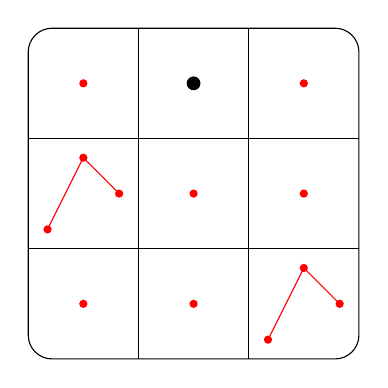
\begin{tikzpicture}[scale=0.7, every node/.style={scale=0.7}]
    \def\spnt{0.075} % Size of smaller points
    \def\lpnt{0.125} % Size of larger points
    \draw[rounded corners=2ex] (0,0) rectangle (6,6);
    \draw (2.0, 6) -- (2.0, 0);
    \draw (4.0, 6) -- (4.0, 0);
    \draw (0, 2) -- (6.0, 2);
    \draw (0, 4) -- (6.0, 4);
    \fill[red] (1, 5) circle (\spnt);
    \fill[red] (1, 1) circle (\spnt);
    \fill[red] (3, 3) circle (\spnt);
    \fill[red] (3, 1) circle (\spnt);
    \fill[red] (5, 5) circle (\spnt);
    \fill[red] (5, 3) circle (\spnt);
    \fill (3,5) circle (\lpnt);
    \draw[red] (0.25+0.1, 2.25+0.1) -- (1,3.75-0.1) -- (1.75-0.1,3);
    \draw[red] (4.25+0.1, 0.25+0.1) -- (5,1.75-0.1) -- (5.75-0.1,1);
    \fill[red] (0.25+0.1, 2.25+0.1) circle (\spnt);
    \fill[red] (1,3.75-0.1) circle (\spnt);
    \fill[red] (1.75-0.1,3) circle (\spnt);
    \fill[red] (4.25+0.1, 0.25+0.1) circle (\spnt);
    \fill[red] (5,1.75-0.1) circle (\spnt);
    \fill[red] (5.75-0.1,1) circle (\spnt);
\end{tikzpicture}